\documentclass[11pt,a4paper]{article}
\usepackage[spanish,es-nodecimaldot]{babel}	% Utilizar español
\usepackage[utf8]{inputenc}					% Caracteres UTF-8
\usepackage{graphicx}						% Imagenes
\usepackage[hidelinks]{hyperref}			% Poner enlaces sin marcarlos en rojo
\usepackage{fancyhdr}						% Modificar encabezados y pies de pagina
\usepackage{float}							% Insertar figuras
\usepackage[textwidth=390pt]{geometry}		% Anchura de la pagina
\usepackage[nottoc]{tocbibind}				% Referencias (no incluir num pagina indice en Indice)
\usepackage{enumitem}						% Permitir enumerate con distintos simbolos
\usepackage[T1]{fontenc}					% Usar textsc en sections
\usepackage{amsmath}						% Símbolos matemáticos

% Comando para poner el nombre de la asignatura
\newcommand{\asignatura}{Asignatura}
\newcommand{\autor}{Vladislav Nikolov Vasilev}
\newcommand{\titulo}{Trabajo 2}
\newcommand{\subtitulo}{Cuestiones de teoría}

\newcommand{\answer}{\noindent\textbf{Solución}}
\newcommand{\question}[1]{\noindent\textbf{#1}}
\newcommand{\nonumsection}[1]{\section*{#1}\addcontentsline{toc}{section}{#1}}

% Configuracion de encabezados y pies de pagina
\pagestyle{fancy}
\lhead{\autor{}}
\rhead{\asignatura{}}
\lfoot{Grado en Ingeniería Informática}
\cfoot{}
\rfoot{\thepage}
\renewcommand{\headrulewidth}{0.4pt}		% Linea cabeza de pagina
\renewcommand{\footrulewidth}{0.4pt}		% Linea pie de pagina

\begin{document}
\pagenumbering{gobble}

% Pagina de titulo
\begin{titlepage}

\begin{minipage}{\textwidth}

\centering

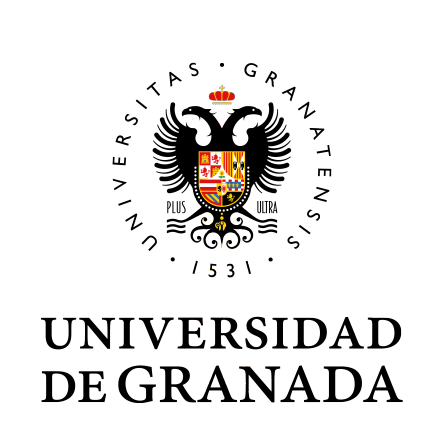
\includegraphics[scale=0.5]{img/ugr.png}\\

\textsc{\Large \asignatura{}\\[0.2cm]}
\textsc{GRADO EN INGENIERÍA INFORMÁTICA}\\[1cm]

\noindent\rule[-1ex]{\textwidth}{1pt}\\[1.5ex]
\textsc{{\Huge \titulo\\[0.5ex]}}
\textsc{{\Large \subtitulo\\}}
\noindent\rule[-1ex]{\textwidth}{2pt}\\[3.5ex]

\end{minipage}

\vspace{0.5cm}

\begin{minipage}{\textwidth}

\centering

\textbf{Autor}\\ {\autor{}}\\[2.5ex]
\textbf{Rama}\\ {Computación y Sistemas Inteligentes}\\[2.5ex]
\vspace{0.3cm}


\includegraphics[scale=0.3]{img/etsiit.jpeg}

\vspace{0.7cm}
\textsc{Escuela Técnica Superior de Ingenierías Informática y de Telecomunicación}\\
\vspace{1cm}
\textsc{Curso 2019-2020}
\end{minipage}
\end{titlepage}

\pagenumbering{arabic}
\tableofcontents
\thispagestyle{empty}				% No usar estilo en la pagina de indice

\newpage

\setlength{\parskip}{1em}

\nonumsection{Ejercicio 1}

\question{Identifique las semejanzas y diferencias entre los problemas
de: a) clasificación de imágenes; b) detección de objetos: c)
segmentación de imágenes; d) segmentación de instancias.}

\answer

\nonumsection{Ejercicio 2}

\question{¿Cuál es la técnica de búsqueda estándar para la detección de
objetos en una imagen? Identifique pros y contras de la misma e
indique posibles soluciones para estos últimos.}

\answer

\nonumsection{Ejercicio 3}

\question{Considere la aproximación que extrae una serie de
características en cada píxel de la imagen para decidir si hay
contorno o no. Diga si existe algún paralelismo entre la forma de
actuar de esta técnica y el algoritmo de Canny. En caso positivo
identifique cuales son los elementos comunes y en que se diferencian
los distintos.}

\answer

\nonumsection{Ejercicio 4}

\question{Tanto el descriptor de SIFT como HOG usan el mismo tipo de
información de la imagen pero en contextos distintos. Diga en que se
parecen y en que son distintos estos descriptores. Explique para que
es útil cada uno de ellos.}

\answer

\nonumsection{Ejercicio 5}

\question{Observando el funcionamiento global de una CNN, identifique que
dos procesos fundamentales definen lo que se realiza en un pase hacia
delante de una imagen por la red. Asocie las capas que conozca a cada
uno de ellos.}

\answer

\nonumsection{Ejercicio 6}

\question{Se ha visto que el aumento de la profundidad de una CNN es un
factor muy relevante para la extracción de características en
problemas complejos, sin embargo este enfoque añade nuevos problemas.
Identifique cuales son y qué soluciones conoce para superarlos.}

\answer

\nonumsection{Ejercicio 7}

\question{Existe actualmente alternativas de interés al aumento de la
profundidad para el diseño de CNN. En caso afirmativo diga cuál/es y
como son.}

\answer

\nonumsection{Ejercicio 8}

\question{Considere una aproximación clásica al reconocimiento de escenas
en donde extraemos de la imagen un vector de características y lo
usamos para decidir la clase de cada imagen. Compare este
procedimiento con el uso de una CNN para el mismo problema. ¿Hay
conexión entre ambas aproximaciones? En caso afirmativo indique en
que parecen y en que son distintas.}

\answer

\nonumsection{Ejercicio 9}

\question{¿Cómo evoluciona el campo receptivo de las neuronas de una CNN
con la profundidad de la capas? ¿Se solapan los campos receptivos de
las distintas neuronas de una misma profundidad? ¿Es este hecho algo
positivo o negativo de cara a un mejor funcionamiento?}

\answer

\nonumsection{Ejercicio 10}

\question{¿Qué operación es central en el proceso de aprendizaje y
optmización de una CNN?}

\answer

\nonumsection{Ejercicio 11}

\question{Compare los modelos de detección de objetos basados en
aproximaciones clásicas y los basados en CNN y diga que dos procesos
comunes a ambos aproximaciones han sido muy mejorados en los modelos
CNN. Indique cómo.}

\answer

\nonumsection{Ejercicio 12}

\question{Es posible construir arquitecturas CNN que sean independientes
de las dimensiones de la imagen de entrada. En caso afirmativo diga
cómo hacerlo y cómo interpretar la salida.}

\answer

\nonumsection{Ejercicio 13}

\question{Suponga que entrenamos una arquitectura Lenet-5 para clasificar
imágenes $128 \times 128$ de 5 clases distintas. Diga que cambios deberían de
hacerse en la arquitectura del modelo para que se capaz de detectar
las zonas de la imagen donde aparecen alguno de los objetos con los
que fue entrenada.}

\answer

\nonumsection{Ejercicio 14}

\question{Argumente por qué la transformación de un tensor de dimensiones
$128 \times 32 \times 32$ en otro de dimensiones $256 \times 16 \times 16$,
usando una convolución $3 \times 3$ con stride=2, tiene sentido que pueda
ser aproximada por una secuencia de tres convoluciones: convolución $1 \times 1$
+ convolución $3 \times 3$ + convoluión $1 \times 1$. Diga también qué papel
juegan cada una de las tres convoluciones.}

\answer

\nonumsection{Ejercicio 15}

\question{Identifique una propiedad técnica de los modelos CNN que permite
pensar que podrían llegar a aproximar con precisión las
características del modelo de visión humano, y que sin ella eso no
sería posible. Explique bien su argumento.}

\answer

\newpage

\begin{thebibliography}{5}

\bibitem{nombre-referencia}
Texto referencia
\\\url{https://url.referencia.com}

\end{thebibliography}

\end{document}

